\documentclass[twoside]{hcmut-report}
\usepackage{matlab-prettifier}
\parindent 0pt

% Sub-preambles
% https://github.com/MartinScharrer/standalone
% colors
\definecolor{mygreen}{HTML}{5CAA5C}
\DeclareMathOperator\caret{\raisebox{1ex}{$\scriptstyle\wedge$}}

% Encodings
\usepackage{gensymb,textcomp}

% Better tables
% Wide tables go to https://tex.stackexchange.com/q/332902
\usepackage{array,multicol,multirow,siunitx,tabularx}

% Better enum
\usepackage{enumitem}

% Graphics
\usepackage{caption,float}

% Configurations
\title{Calculus 2 Assignment}
\reporttype{Instructor: Dau The Phiet}

\usepackage{tocloft}
\renewcommand{\thesection}{\Roman{section}}
\renewcommand{\thesubsection}{\thesection.\Roman{subsection}}
\renewcommand{\cftsecaftersnum}{. }

% Custom commands
\newcommand*\mean[1]{\bar{#1}}

\begin{document}
\coverpage%

\tableofcontents
\clearpage

%% ============ SECTION 1 ============ %%
\section{ Problem 1.}
\textit{
  Let $ z = f(x) = x^2 + 2y^2 + 3xy^3 - y^3 $.
  \begin{enumerate}[label=(\alph*)]
    \item Draw the graph of the function.
    \item Draw the contour plot of the function. Point out the local extreme
    and the saddle point on that figure.
    \item Find the exact local extreme and saddle point (using calculus
    technique).
  \end{enumerate}
}

\vspace*{1cm}

\textbf{Theory: }\\
We all know that the main uses of ordinary derivatives are to find maximum and minimum values (extreme values). Similar with multivariable functions, we can use partial derivatives to do the same thing.\\
Suppose we have a two-variable function $f$ that is continuous on the interval $(a,b)$ and it is said that:\\[6pt]
A function $f$ of two variables has a local maximum at $(a,b)$ if $f(x,y) \leq f(a,b)$ when $(x,y)$ is near $(a,b)$.
This means that $f(x,y) \leq f(a,b)$ for all points $(x,y)$ in some disk with center $(a,b)$. The number $f(a,b)$ is called a local maximum value. If $f(x,y) \geq f(a,b)$ when $(x,y)$ is near $(a,b)$, then $f$ has a local minimum at $(a,b)$ and $f(a,b)$ is a local minimum value.\\[6pt]
If the inequalities in the above definition hold for all points $(x,y)$ in the domain of $f$, then $f$ has an absolute maximum or local minimum at $(a,b)$.\\
Therefore, If $f$ has a local maximum or minimum at $(a,b)$ and the first-order partial derivatives of $f$ exist at that point, then $f_x(a,b) = 0$ and $f_y(a,b)=0$.\\[6pt]
But in some problems, There's a point called saddle point which located at the origin. Thus, we have another tool called \textbf{Second Derivatives Test} to determine which points are minimum, maximum and saddle.\\[6pt]
Assume that the second partial derivatives are continuous on a disk with center $(a,b)$, and suppose $f_x(a,b)=0$ and $f_y(a,b)=0$. Let:
$$ D(a,b) = f_{xx}(a,b) f_{yy}(a,b) - [f_{xy}(a,b)]^2 $$
If $D>0$ and $f_{xx}(a,b)>0$, then $f(a,b)$ is a local minimum.\\
If $D>0$ and $f_{xx}(a,b)<0$, then $f(a,b)$ is a local minimum.\\
If $D<0$, then $f(a,b)$ is not a local extrema, and the point $(a,b)$ is called a saddle point of $f$.\\
\textbf{Note}: If $D=0$, the test tells no information. $f$ could have a local maximum or local minimum at $(a,b)$, or $(a,b)$ could be a saddle point of $f$.\\

Finding the local extreme values of the function $f(x,y)$:
\begin{itemize}
  \item Identifying critical points for the given function $f(x,y)$.
    \begin{itemize}
      \item Find the partial derivatives with respect to $x$ and to $y$.
      \item Set each partial derivative equal to zero.
      \item Solve the system of equations to get critical points $(x_0,y_0)$.
    \end{itemize}

  \item Consider $D(x_0,y_0)$.
    \begin{itemize}
      \item Find all second derivatives of $f(x_0,y_0)$.
      \item Identify by the Second Derivative Test $ D(a,b) = f_{xx}(a,b) f_{yy}(a,b) - [f_{xy}(a,b)]^2 $
    \end{itemize}
\end{itemize}

\vspace*{1cm}

\textbf {Hand-writing solution: }\\[6pt]
Find the local extreme values of the function $f(x,y) = x^2 + 2y^2 + 3xy^3 - y^3 $:\\[6pt]
Firstly, we have to determine critical points for the given function $f(x,y)$ by finding the partial derivatives with respect to $x$ and to $y$ and set each partial derivative equal to zero.
$$ f_x = 2x + 3y^3 $$
$$ f_y = 4y + 9xy^2 - 3y^2 $$
We then have the system of equations:
\[
\begin{cases}
  2x + 3y^3 &= 0 \qquad (1) \\
  4y + 9xy^2 - 3y^2 &= 0 \qquad (2)
\end{cases}
\]
Solve the equation (1) for $x$:
$$ x = -\dfrac{3}{2} y^3 \qquad (4)$$
Substitute that value to the equation (2):
$$ 4y + 9\left( -\dfrac{3}{2} y^3 \right)y^2 - 3y^2 = 0 $$
Simplify the above equation:
$$ y\left( -\dfrac{27}{2}y^4 - 3y + 4 \right) = 0 $$
Solve the equation for $y$ and substitute the value to the equation (4):
\begin{align*}
  y = 0 &\Rightarrow x = 0 \\
  y = 0.629 &\Rightarrow x = -0.373 \\
  y = -0.833 &\Rightarrow x = 0.867 
\end{align*}
Thus, we have three critical points: $(0,0), (-0.373, 0.629), (0.867, -0.833)$.\\[6pt]
Next step is to consider $D(x_0,y_0)$ by finding all second derivatives of $f(x_0,y_0)$ and identify by the Second Derivative Test 
$$ D(x_0,y_0) = f_{xx}(x_0,y_0) f_{yy}(x_0,y_0) - [f_{xy}(x_0,y_0)]^2 $$
We have:
\begin{align*}
  f_{xx} &= 2 \\
  f_{yy} &= 4 + 18xy - 6y \\
  f_{xy} &= 9y^2
\end{align*}
Therefore:
$$ D(x_0,y_0) = -81y^4+36xy-12y+8 \qquad (5)$$
Then, we substitute 3 critical points into equation (5) in turn.
\begin{itemize}
  \item At $ (0,0) $:
    \begin{itemize}
      \item $ D(0,0) = 8 > 0 $
      \item $ f_{yy}(0,0) = 2 > 0$
    \end{itemize}
    $\Rightarrow f(0,0)$ is a local minimum.
  \item At $ (-0.373, 0.629) $:
    \begin{itemize}
      \item $ D(-0.373, 0.629) = -20.678 < 0 $
    \end{itemize}
    $\Rightarrow (-0.373, 0.629)$ is a saddle point of $f$.
  \item At $ (0.867, -0.833) $  
    \begin{itemize}
      \item $ D(0.867, -0.833) = -46.993 < 0 $
    \end{itemize}
    $\Rightarrow (0.867, -0.833)$ is a saddle point of $f$.
\end{itemize}

\vspace*{1cm}

\textbf {MATLAB code: }
\begin{lstlisting}[style=Matlab-editor]
    %calculation
    syms x y z
    z = x.^2 + 2*y.^2 + 3*x.*y.^3 - y.^3;
    
    %differentiate z 
    fx = diff(z,x,1);   
    fy = diff(z,y,1);
    fxx = diff(z,x,2);
    fyy = diff(z,y,2);
    fxy = diff(fx,y,1);
    
    %create a system equation
    eqns = [ fx == 0, fy == 0];
    
    %define the variables for system equation
    vars = [x y];
    
    %solve the system equation
    [solx, soly] = vpasolve(eqns, vars);
    
    %only choose the real value
    solx_real = solx(imag(solx)==0);
    soly_real = soly(imag(solx)==0);
     
     
    %display section
    disp(['z = f(x,y) = ', char(z)])
    disp(['fx = ', char(fx)])
    disp(['fy = ', char(fy)])
    disp(['fxx = ', char(fxx)])
    disp(['fyy = ', char(fyy)])
    disp(['fxy = ', char(fxy)])
     
    %c
    for n=1:length(solx_real)
        fxx_val = subs(fxx,[x,y],[solx_real(n),soly_real(n)]);
    
    %calculate fxx, fyy, fxy values
    fyy_val = subs(fyy,[x,y],[solx_real(n),soly_real(n)]);
    fxy_val = subs(fxy,[x,y],[solx_real(n),soly_real(n)]);
    D = fxx_val*fyy_val - fxy_val*fxy_val;
    
    fprintf('\nFor point(%s,%s)\n',solx_real(n),soly_real(n))
        if D > 0
            fprintf('D = fxx*fyy-fxy^2 = %s\n',D)
            fprintf('So D > 0\n')
            fprintf('Therefore point (%s,%s) is local extreme\n',solx_real(n),soly_real(n))
            if fxx_val > 0
                fprintf('And fxx = %s\n',fxx_val)
                fprintf('So fxx > 0\n')
                fprintf('Therefore this is a local minimum point\n')
            else
                fprintf('And fxx = %s\n',fxx_val)
                fprintf('So fxx < 0\n')
                fprintf('Therefore this is a local maximum point\n')
            end
        elseif D < 0
            fprintf('D = fxx*fyy-fxy^2 = %s\n',D)
            fprintf('So D < 0\n')
            fprintf('Therefore point (%s,%s) is a saddle point\n',solx_real(n),soly_real(n))
        else
            fprintf('D = fxx*fyy-fxy^2 = %s\n',D)
            fprintf('So conclusion for point (%s,%s) \n',solx_real(n),soly_real(n))
        end
    end    
\end{lstlisting}

Code explanation: 
\begin{itemize}
  \item \texttt{\color{mygreen}syms x y z;} - declares symbolic variables x, y, and z to be used.
  \item \texttt{\color{mygreen}z = x.$\caret$2 + 2*y.$\caret$2 + 3*x.*y.$\caret$3 - y.$\caret$3;} - defines a symbolic expression for z as a function of x and y.
  \item \texttt{\color{mygreen}fx = diff(z,x,1);} - calculates the first partial derivative of z with respect to x and assigns it to the variable \texttt{\color{mygreen}fx}. Similar for \texttt{\color{mygreen}fy, fxx, fyy} and \texttt{\color{mygreen}fxy}.
  \item \texttt{\color{mygreen}eqns = [ fx == 0, fy == 0];} - creates a system of equations eqns that must be solved simultaneously, which are the first-order partial derivative equations set to zero.
  \item \texttt{\color{mygreen}vars = [x y];} - defines the variables to be solved for as x and y.
  \item \texttt{\color{mygreen}[solx, soly] = vpasolve(eqns, vars);} - solves the system of equations eqns for the variables vars and returns the solutions in the vectors solx and soly.
  \item \texttt{\color{mygreen}solx\_real = solx(imag(solx)==0);} - extracts the real parts of the solutions for solx and assigns them to solx\_real.
  \item \texttt{\color{mygreen}disp(['z = f(x,y) = ', char(z)]);} - displays the symbolic expression for z as a function of x and y.
  \item \texttt{\color{mygreen}for n=1:length(solx\_real)} - starts a loop over the number of real solutions found.
  \item \texttt{\color{mygreen}fxx\_val = subs(fxx,[x,y],[solx\_real(n),soly\_real(n)]);} - substitutes the values of solx\_real(n) and soly\_real(n) into the symbolic expression for fxx and assigns the resulting value to fxx\_val.
  \item \texttt{\color{mygreen}vpasolve();} - function is used to solve the system of equations eqns for the variables vars, which are x and y in this case.
  \item \texttt{\color{mygreen}fprintf()} - displays the results of the calculations.
\end{itemize}

\begin{figure}[H]
  \centering
  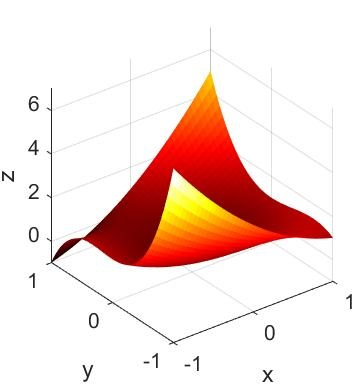
\includegraphics[width=12cm]{graphics/1a.jpg}
  \caption{The graph of the function $ z = f(x) = x^4 - 2x^2 - y^3 + 3y $.}
\end{figure}

\begin{lstlisting}[style=Matlab-editor]
    syms x y z
    [x,y] = meshgrid(-1:0.05:1,-1:0.05:1);
    z = x.^2 + 2*y.^2 + 3*x.*y.^3 - y.^3;

    %plot 2 figure in 1 window
    tiledlayout(2,1);

    %a
    nexttile
    surf(x,y,z,'edgecolor', 'none');
    colormap hot;   %the higher value, the hotter color
    xlabel('x');
    ylabel('y');
    zlabel('z');
    title('GRAPH OF THE FUNCTION')
    pbaspect([1,1,1])

    %b
    nexttile
    contour(x,y,z,200)
    hold on
    for n =1:length(solx_real)
        plot(solx_real(n),soly_real(n),'*')
    end
    xlabel('x');
    ylabel('y');
    title({'CONTOUR PLOT THE FUNCTION,','LOCAL EXTREME AND SADDLE POINT'})
    pbaspect([1,1,1])
\end{lstlisting}

\begin{figure}[H]
  \centering
  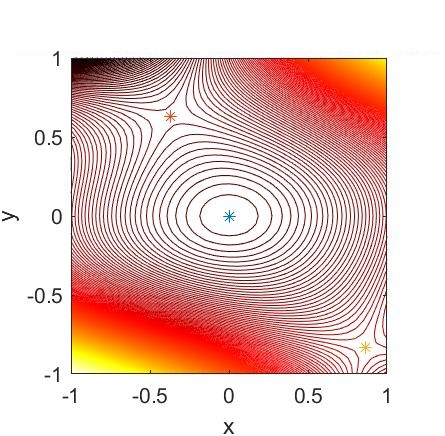
\includegraphics[width=12cm]{graphics/1b.jpg}
  \caption{The contour plot the function $ z = f(x) = x^4 - 2x^2 - y^3 + 3y $.}
\end{figure}

Code explanation: 
\begin{itemize}
  \item \texttt{\color{mygreen}meshgrid()} - generate a grid of x and y values to plot the surface and contour plots of the function.
  \item \texttt{\color{mygreen}tiledlayout()} - create a tiled layout for plotting multiple figures in one window.
  \item \texttt{\color{mygreen}nexttile()} - specify the location of the next plot in the tiled layout. 
  \item \texttt{\color{mygreen}surf()} - create a surface plot of the function.
  \item \texttt{\color{mygreen}colormap()} - set the colormap for the surface plot.
  \item \texttt{\color{mygreen}title()} - add title to the plot
  \item \texttt{\color{mygreen}contour()} - create a contour plot of the function. It takes x, y, and z matrices as input, and creates contour lines at different function values.
  \item \texttt{\color{mygreen}hold on} - allow multiple plots to be overlaid on top of each other.
  \item \texttt{\color{mygreen}for loop} - plot the location of the local extreme and saddle points on the contour plot.
  \item \texttt{\color{mygreen}pbaspect()} - set the aspect ratio of the plot.
\end{itemize}

\vspace*{2cm}

%% ============ SECTION 2 ============ %%
\newpage
\section{ Problem 2.}
\textit{
  Find the maximum and minimum values of $ z = 2x^2 - 2xy + y^3 $ subject to the single constraint $ x^2 + y^2 = 4 $.
  \begin{enumerate}[label=(\alph*)]
    \item Using Lagrange multiplier method.
    \item Using contour plot (Draw the contour plot of the function and
    the constraint curve in the same figure).  
  \end{enumerate}
}

\vspace*{1cm}

\textbf{Theory: }

To find the maximum and minimum value of $f(x,y) = 2x^2 - 2xy + y^3$ subject to the single constraint $ g(x,y) = x^2 + y^2 = 4 $, we need to use the Lagrange multiplier method.\\

Lagrange multiplier method is a technique for finding maximum or minimum values of some multivariable function $f(x,y,z, ...)$ subject to a constraint of the form $g(x,y,z,...)$.\\

For example, a function of 2 variables can be used to explain the method. We get started by finding the extreme values of $f(x,y)$ subject to a constraint $g(x,y)$. In other words, we find the points satisfying the condition that points $(x,y)$ lie on the level curve $g(x,y)=k$.  The figure below shows this curve together with several level curves of $f(x,y)$. These have the equations $f(x,y) = c$  where  $c \in \{7,8,9,10,11\}$.

\begin{figure}[H]
  \centering
  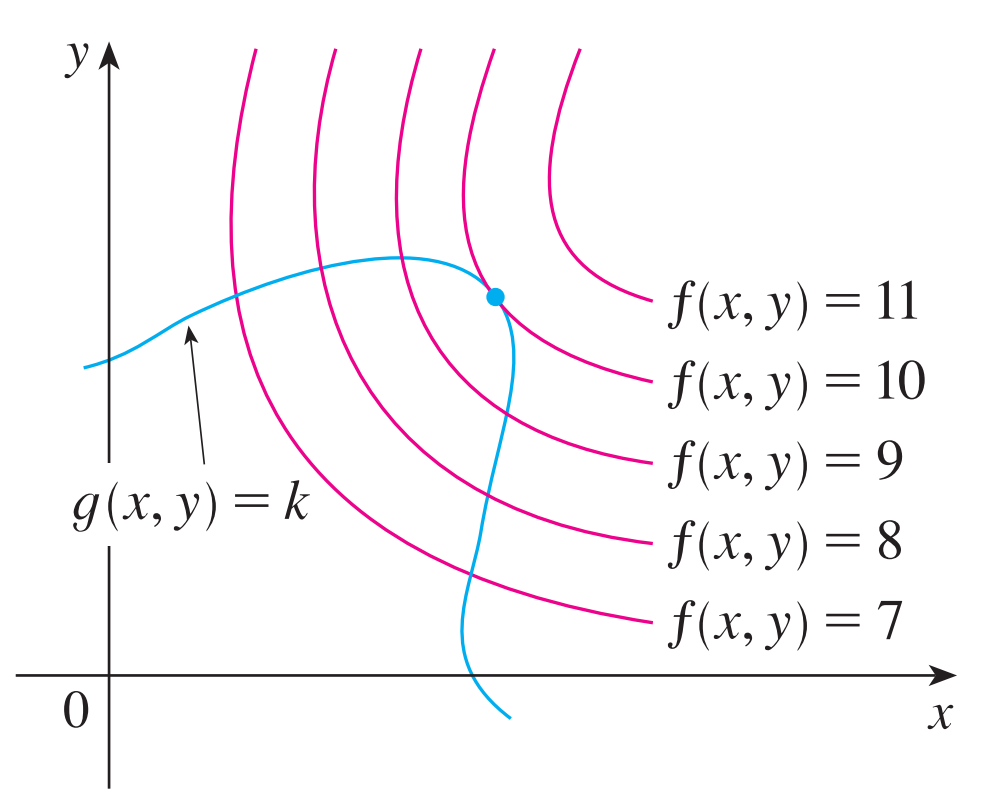
\includegraphics[width=9cm]{graphics/2a.png}
  % \caption{}
\end{figure}

The graph illustrates that the maximum value occupied at the point where $f(x,y)=10$ intersecting $g(x,y)=k$. Analyzing the graph, we can easily see the fact that the maximum value appears when those 2 functions touch each other and they have the same tangent line. Thus the normal lines at the point of intersection $(x_0,y_0)$ are identical. So the gradient vectors are parallel; Therefore, $\nabla f(x_0,y_0) = \lambda g(x_0,y_0)$ where $\lambda$ is a scalar. \\[6pt]
For some scalar $\lambda$. The scalar parameter is called a Lagrange multiplier. The procedure based on the above equation is as follows. We have from the chain rule,
$$ \dfrac{df(x, y)}{dxdy} = \dfrac{\partial f(x, y)}{\partial x} dx + \dfrac{\partial f(x, y)}{\partial y} = 0,\quad \dfrac{dg(x, y)}{dxdy} = \dfrac{\partial g(x, y)}{\partial x} dx + \dfrac{\partial g(x, y)}{\partial y} $$ \\[6pt]
Multiplying the second equation by $\lambda$ and then add to first equation yield:
$$ \left( \dfrac{\partial f(x, y)}{\partial x} + \dfrac{\partial g(x, y)}{\partial x} \right)dx + \left( \dfrac{\partial f(x, y)}{\partial y} + \dfrac{\partial g(x, y)}{\partial y} \right)dy = 0 $$\\[6pt]
Then we can rewrite the expression as the vector equation:
$$ \nabla f(x_0, y_0) =\lambda \nabla g(x_0, y_0) $$
Thus, the maximum and minimum values of $f(x,y)$ subject to the constraint $g(x_0,y_0)=0$  can be found by solving the following set of equations.
$$ \dfrac{\partial f(x, y)}{\partial x} + \dfrac{\partial g(x, y)}{\partial x} = 0 $$
$$ \dfrac{\partial f(x, y)}{\partial y} + \dfrac{\partial g(x, y)}{\partial y} = 0 $$
$$ g(x, y) = 0 $$\\[6pt]
The Lagrange multiplier method allows us to find the values of the variables that optimize the objective function subject to the given constraints. This technique is widely used in various fields of mathematics, physics, and engineering, particularly in optimization problems involving constraints.\\[6pt]

\textbf{Solving Problem using Lagrange multiplier method:}\\[6pt]
$$ Let \quad  f(x,y)= z = 2x^2-2xy+y^3 \quad and \quad g(x,y)=x^2 + y^2- 4 $$
Therefore, we obtain a system of equations:
\[
\begin{cases}
  x - 2y + 2 \lambda x &= 0 \qquad (1) \\
  2x + 3y^2 + 2 \lambda x &= 0 \qquad (2) \\
  x^2 + y^2 - 4 &= 0 \qquad (3) \\
\end{cases}
\]

Solve the equation $(1)$ for $x$, we get:
$$ x = \dfrac{y}{2 + \lambda} $$

Substitute $x$ in the equation $(2)$:
$$ 3y^2 + 2 \lambda y - \dfrac{2y}{2 + \lambda} = 0 \quad (4)$$

Then we substitute $x$ into the equation $(3)$ and solve for $y$:
\begin{align*}
  \dfrac{y^2}{(2 + \lambda)^2} + y^2 &= 4 \\
  y^2 &= \dfrac{4}{1 + \dfrac{1}{(2 + \lambda)^2}} \\
  y &= \pm \dfrac{2}{  \sqrt{1 + \dfrac{1}{(2+ \lambda)^2}}  } \\
\end{align*}

Plug $y = -\dfrac{2}{  \sqrt{1 + \dfrac{1}{(2+ \lambda)^2}}  }$ to equation $(4)$ then we obtain:
$$ 3 \dfrac{4}{1 + \dfrac{1}{(2+x)^2}} + 2 \lambda \dfrac{-2}{ \sqrt{1 + \dfrac{1}{(2 + \lambda)^2}} } - \dfrac{-4}{(2 + \lambda) \sqrt{1 + \left(\frac{1}{2 + \lambda}\right)^2} } = 0 $$\\[6pt]

Then we obtain 2 values of $\lambda$:
$$ \lambda = 3.13935 \quad and \quad \lambda = -2.31197 $$

With $y = \dfrac{2}{  \sqrt{1 + \dfrac{1}{(2+ \lambda)^2}}  }$ we have another equation:
$$ 3 \dfrac{4}{1 + \dfrac{1}{(2+x)^2}} + 2 \lambda \dfrac{2}{ \sqrt{1 + \dfrac{1}{(2 + \lambda)^2}} } - \dfrac{4}{(2 + \lambda) \sqrt{1 + \left(\frac{1}{2 + \lambda}\right)^2} } = 0 $$\\[6pt]

Also, two other values of $\lambda$:
$$ \lambda = -1,03873 \quad and \quad \lambda = -3.1317 $$

Last step is to compute value of $x$ and $y$ according to each value of $\lambda$: \\
With $\lambda = 3.13935$:
$$ y = -\dfrac{2}{ \sqrt{1 + \dfrac{1}{(2 + \lambda)^2}} } = -\dfrac{2}{ \sqrt{1 + \dfrac{1}{(2 + 3.13935)^2}} } = -1.96318$$
$$ x = \dfrac{y}{2 + \lambda} = \dfrac{-1.96318}{2 + 3.13935} = -0.38199 $$

With $\lambda = -2.31197$: 
$$ y = -\dfrac{2}{ \sqrt{1 + \dfrac{1}{(2 + \lambda)^2}} } = -\dfrac{2}{ \sqrt{1 + \dfrac{1}{(2 -2.31197)^2}} } = -0.595631$$
$$ x = \dfrac{y}{2 + \lambda} = \dfrac{-0.595631}{2 -2.31197} = 1.90925 $$

With $\lambda = -1,03873$: 
$$ y = -\dfrac{2}{ \sqrt{1 + \dfrac{1}{(2 + \lambda)^2}} } = -\dfrac{2}{ \sqrt{1 + \dfrac{1}{(2 -1,03873)^2}} } =1.38602$$
$$ x = \dfrac{y}{2 + \lambda} = \dfrac{1.38602}{2 -1,03873} = 1.44186 $$

With $\lambda =-3.13172$: 
$$ y = -\dfrac{2}{ \sqrt{1 + \dfrac{1}{(2 + \lambda)^2}} } = -\dfrac{2}{ \sqrt{1 + \dfrac{1}{(2 -3.13172)^2}} } = 1.49874$$
$$ x = \dfrac{y}{2 + \lambda} = \dfrac{1.49874}{2 -3.13172} = -1.3243 $$\\[6pt]
After obtaining all value of $x, y$ in each case of $\lambda$, we evaluate $f$ at all the point $(x,y)$. The largest of those values is the maximum value of $f$; the smallest is the minimum value of $f$.
\begin{align*}
  f(-0.38199,-1.96318)
    &=2(-0.38199)^2-2(-0.38199)(-1.96318)+(-1.96318)^3\\
    &=-8.77424\\[6pt]
  f(1.90925,-0.595631)
    &=2(1.90925)^2-2(1.90925)(-0.595631)+(-0.595631)^3\\
    &=9.35357\\[6pt]
  f(1.44186,1.38602)
    &=2(1.44186 )^2-2(1.44186 )(1.38602)+(1.38602)^3\\
    &=2.82364\\[6pt]
  f(-1.3243,1.49874)
    &=2(-1.3243 )^2-2(-1.3243 )(1.49874)+(1.49874)^3\\
    &=10.8436\\[6pt]
\end{align*}

\textit{Therefore: }
\begin{itemize}
  \item Maximum value of $z = 2x^2 - 2xy + y^3$ subject to the single constraint $x^2 + y^2 = 4$ is \\
        $f(-1.3243,1.49874) = 10.8436$
  \item Minimum value of $z = 2x^2 - 2xy + y^3$ subject to the single constraint $x^2 + y^2 = 4$ is \\
        $f-0.38199,-1.96318=-8.77424$
\end{itemize}

\textbf{MATLAB code: }
This MATLAB code demonstrates how to plot the contour of a function and a constraint curve in the same figure. Specifically, the function is $z = 2x^2-2xy+y^3$ and the constraint curve $x^2 + y^2 = 4$ in the same figure.

\begin{lstlisting}[style=Matlab-editor]
  % Define the range of values for x and y
  x = linspace(-5, 5, 100);
  y = linspace(-5, 5, 100);
  
  % Create a grid of x and y values
  [X, Y] = meshgrid(x, y);
  
  % Evaluate the function z at each point on the grid
  Z = 2*X.^2 - 2*X.*Y + Y.^3;
  
  % Plot the contour of the function
  contour(X, Y, Z, 100);
  hold on
  
  % Plot the constraint x^2 + y^2 = 4
  theta = linspace(0, 2*pi, 100);
  r = 2; % set the radius of the circle
  x_circle = r*cos(theta); % compute x coordinates
  y_circle = r*sin(theta); % compute y coordinates
  plot(x_circle, y_circle, 'k','Color','red', 'LineWidth', 2)
  
  % Set labels
  xlabel('x');
  ylabel('y');
  title('Contour plot of z = 2x^2 - 2xy + y^3 and constraint x^2 + y^2 = 4');
  
  % Adjust the aspect ratio of the plot
  pbaspect([1 1 1])  
\end{lstlisting}

\begin{figure}[H]
  \centering
  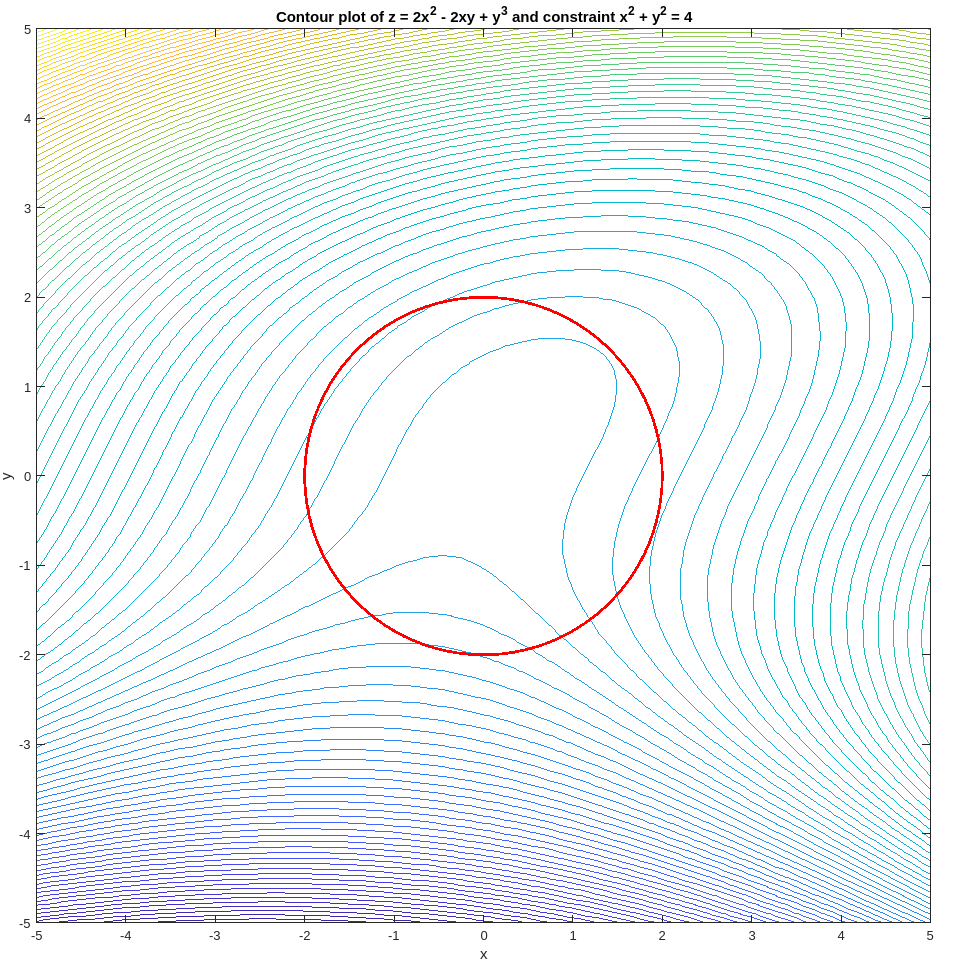
\includegraphics[width=12cm]{graphics/2b.png}
  \caption{The contour plot of the function $z = 2x^2 - 2xy + y^3$ and the constraint $x^2 + y^2 = 4$.}
\end{figure}

\vspace*{1cm}

Code explanation:
\begin{itemize}
  \item \texttt{\color{mygreen}theta = linspace(0, 2*pi, 100)} - create a 1x100 row vector $\theta$ of equally spaced values between 0 and 2$\pi$ radians with 100 elements.
  \item \texttt{\color{mygreen}x\_circle = r*cos(theta)} - compute the x-coordinates of the circle using the $\cos$ function and $\theta$.
  \item \texttt{\color{mygreen}y\_circle = r*sin(theta)} - compute the y-coordinates of the circle using the $\sin$ function and $\theta$.
\end{itemize}

\vspace*{2cm}

%% ============ SECTION 3 ============ %%
\newpage
\section{ Problem 3.}
\textit{
  Let $C$ be the intersection of the surface $x^2 + y^2 + z^2 = 9$ and the cylinder $x^2 + 3y^2 = 4,\quad z > 0$.
  \begin{enumerate}[label=(\alph*)]
    \item Draw the surfaces and the curve $C$.
    \item Find the length of the curve.
    \item At any given point $(x_0, y_0, z_0)$ belongs to the curve, draw the unit tangent vector.  
  \end{enumerate}
}

\vspace*{1cm}

\textbf{Theory: Finding the length of a curve using line integral.} \\
Suppose that a curve $C$ is defined by equation $y=f(x)$, where $f$ is continuous and $a \leq x \leq b$. We obtain a polygonal approximation to $C$ by dividing the interval $[a,b]$ into $n$ subintervals with endpoints $x_0,x_1,...,x_n$ and equal with $\Delta x$. If $y_i=f(x_i)$, and then the point $P_i(x,y)$ lies on $C$ and the polygon with vertices $P_0,P_1,...,P_n$, Illustrated in the below figure, is an approximation to $C$.\\[6pt]
\begin{figure}[H]
  \centering
  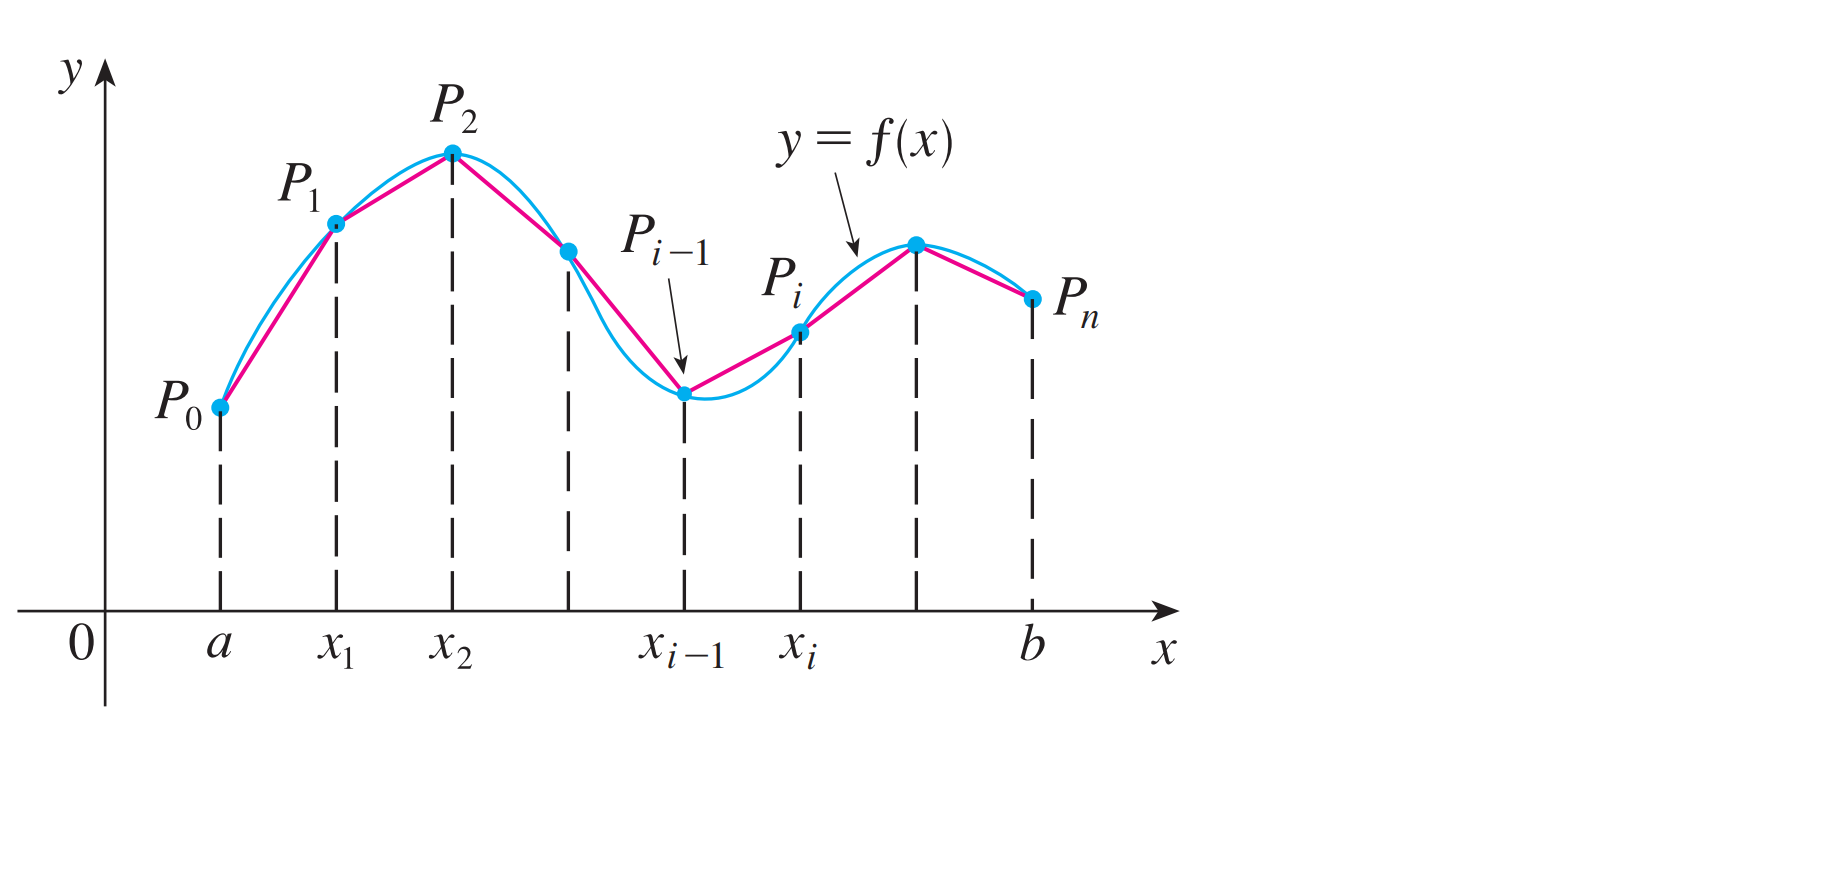
\includegraphics[width=12cm]{graphics/3_0.png}
  % \caption{}
\end{figure}
The length $L$ of is approximately the length of this polygon and the approximation gets better as we let $n$ increase. Therefore we define the length $\mathbf{L}$ of the curve $C$ with equation $y=f(x)$, $a \leq x \leq b$, as the limit of the lengths of these inscribed polygons (if the limit exists):
$$ L = \lim_{n \to \infty} \sum_{i = 1}^{n}  \left| P_{i-1} P_i \right| $$
If we let $\Delta x_i=x_i-x_{i-1}$ and $\Delta y_i=y_i-y_{i-1}$, then
$$ \left| P_{i-1} P_i \right| = \sqrt{(x_i-x_{i-1})^2 + (y_i-y_{i-1})^2} = \sqrt{(\Delta x)^2 + (\Delta y)^2} $$

By applying \textbf{the Mean Value Theorem} to $f$ on the interval $[x_{i-1},x_i]$, we find that there exist a number $x_i*$ between $x_{i-1}$ and $x_i$ such that
$$ f(x_i)-f(x_{i-1})=f(x)(x_i-x_{i-1})$$
$$ \rightarrow \Delta y_i = f'(x_i)\Delta x $$
Thus we have:
$$ \left| P_{i-1} P_i \right| = \sqrt{1^2 + [f'(x)]^2} dx $$
By the definition, this integral exists because the function $g(x) = \sqrt{1^2 + [f'(x)]^2}$ is continuous. Thus we have proved the following theorem:
If $f'$ is continuous on $[a,b]$, then the length of the curve $y=f(x)$, $a \leq x \leq b$, is
$$ L = \int_{a}^{b} \sqrt{1^2 + \left[f'(x)\right]^2} dx  $$

Then we have another assumption that $C$ can be described by the parametric equations $x=f(t)$ and $y=g(t)$, $\alpha \leq x \leq \beta$, where \vspace{0.2cm} $\dfrac{dx}{dt}=f'(t)>0$. This means that $C$ is traversed once, from left to right, as $t$ increased from $\alpha$ to $\beta$ and $f(\alpha)=a, f(\beta)=b$. We obtain:
$$ L = \int_{a}^{b} \sqrt{1^2 + \left[f'(x)\right]^2} dx = \int_{\alpha}^{\beta} \sqrt{\left(\dfrac{dx}{dt}\right)^2 + \left(\dfrac{dy}{dt}\right)^2} dx  $$

The length of space curve is defined in exactly the same way. Suppose that the curve has the vector equation $r(t)=\langle f(t), g(t), h(t) \rangle$, $a\leq x\leq b$, or, equivalently, the parametric equations $x=f(t), y=g(t), z=h(t),$ where $f',g'$ and $h'$ are continuous. If the curve is traversed exactly once as t increases from $a$ to $b$, then it can be shown that its length is
$$ L = \int_{a}^{b} \sqrt{\left[f'(x)\right]^2 + \left[g'(x)\right]^2 + \left[h'(x)\right]^2} dx = \int_{\alpha}^{\beta} \sqrt{\left(\dfrac{dx}{dt}\right)^2 + \left(\dfrac{dy}{dt}\right)^2 + \left(\dfrac{dz}{dt}\right)^2} dx  $$

\vspace*{0.5cm}

\textbf{Tangent vectors: }\\
In mathematics, a tangent vector is a vector that is tangent to a curve or surface at a given point. Tangent vectors are described in the differential geometry of curves in the context of curves in $\mathbb{R}^n$. More generally, tangent vectors are elements of a tangent space of a differentiable manifold. Tangent vectors can also be described in terms of germs. Formally, a tangent vector at the point $x$ is a linear derivation of the algebra defined by the set of germs at $x$.

Let $r(t)$ be a parametric smooth curve. The tangent vector is given by $r'(t)$ where we have used a prime instead of the usual dot to indicate differentiation with respect to parameter $t$. The unit tangent vector is given by
$$ T(x) = \dfrac{r'(x)}{\lvert r(x) \rvert} $$

\vspace*{1cm}

\textbf{MATLAB code: }\\
\textbf{\texttt{a) Draw the surfaces and the curve $C$.} }

\begin{lstlisting}[style=Matlab-editor]
  % Plot the the surface x^2 + y^2 + z^2 = 9
  f = @(x, y, z) x.^2 + y.^2 + z.^2 -9;
  fimplicit3( f , [-3 3 -3 3 0 5 ] , 'c' );  % plot the surface in cyan color
  daspect([1 1 1]) % set the aspect ratio of axes to 1 1 1
  xlabel('x');
  ylabel('y');
  zlabel('z');
  hold on;  % retain the plot for the next plot  
\end{lstlisting}

\begin{figure}[H]
  \centering
  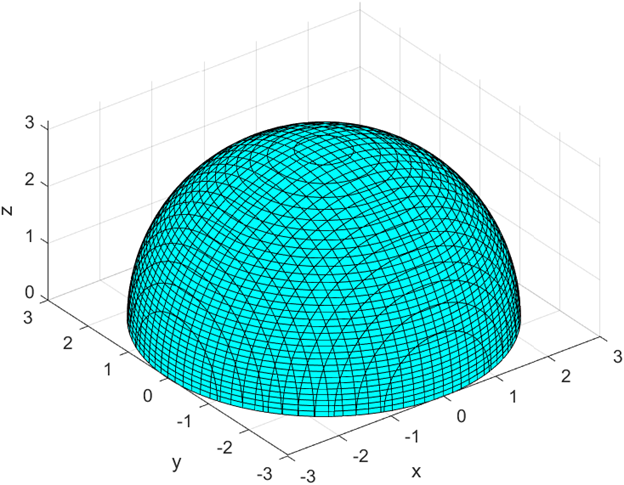
\includegraphics[width=12cm]{graphics/3a1.png}
  \caption{The surface $x^2 + y^2 + z^2 = 9$}
\end{figure}

\begin{lstlisting}[style=Matlab-editor]
% Plot the surface x^2 +3y^2 = 4
g = @(x, y) x.^2 + 3*(y.^2) -4;
fimplicit3 (g, [-3 3 -3 3 0 5 ], 'g');  % plot the surface in green color
daspect([1 1 1]) % set the aspect ratio of axes to 1 1 1
xlabel('x');
ylabel('y');
zlabel('z');
hold on;  % retain the plot for the next plot
\end{lstlisting}

\begin{figure}[H]
  \centering
  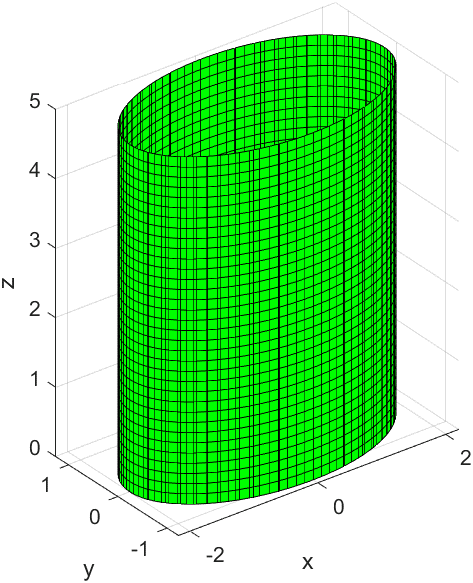
\includegraphics[width=12cm]{graphics/3a2.png}
  \caption{The cylinder $x^2 + 3y^2 = 4$}
\end{figure}

\begin{lstlisting}[style=Matlab-editor]
  % Draw the curve C as the interection of 2 surfaces:
  syms t;
  X = cos(t).*2;
  Y = sin(t).*(2/sqrt(3));
  syms t;
  X = 2.*cos(t) ;
  Y = sin(t).*(2/sqrt(3) );
  Z = sqrt(9 - 4.*cos(t).^2 - 4/3.*sin(t)^2);  % calculate the z-coordinate of the curve
  curveC = fplot3 (X, Y, Z, [ 0 2*pi ], 'linewidth', 5);
  curveC.Color = 'r';  % plot the curve with red color
  daspect([1 1 1]) % set the aspect ratio of axes to 1 1 1
  xlabel('x');
  ylabel('y');
  zlabel('z');
  title("Intersection curve of the surfaces x^2 + y^2 + z^2 = 9 and the cylinder x^2 + 3y^2 = 4, z > 0")   
\end{lstlisting}

\begin{figure}[H]
  \centering
  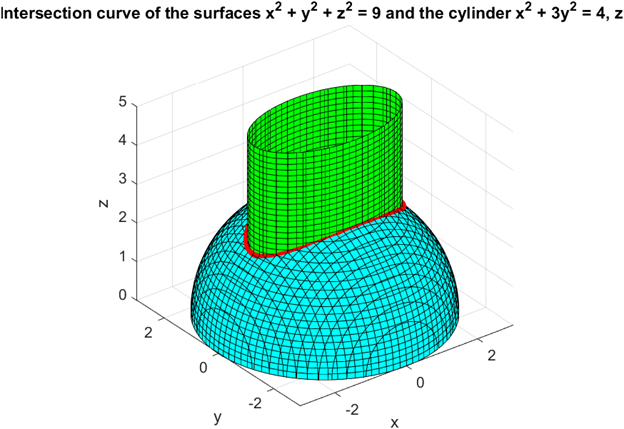
\includegraphics[width=12cm]{graphics/3a3.png}
  \caption{The surfaces and the curve $C$}
\end{figure}

\begin{lstlisting}[style=Matlab-editor]
  % Draw the curve C as the interection of 2 surfaces without line:
  syms t;
  X = cos(t).*2;
  Y = sin(t).*(2/sqrt(3));
  Z = sqrt(9 - 4.*cos(t).^2 - 4/3.*sin(t)^2);  % calculate the z-coordinate of the curve
  curveC = fplot3 (X, Y, Z, [ 0 2*pi ], 'linewidth', 3);
  curveC.Color = 'b';  % plot the curve with blue color
  daspect([1 1 1]) % set the aspect ratio of axes to 1 1 1
  xlabel('x');
  ylabel('y');
  zlabel('z');
  title("The intersection curve C of two surfaces"); 
\end{lstlisting}

\begin{figure}[H]
  \centering
  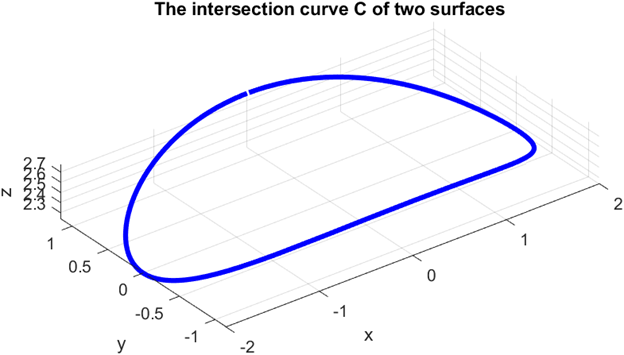
\includegraphics[width=12cm]{graphics/3a4.png}
  \caption{The intersection curve $C$}
\end{figure}

\textbf{ \texttt{b) Find the length of the curve C.} }\\

Solving by hand:\\
First we represent $x$ and $y$ through parameter $t$:
\begin{align}
  \begin{cases}
    x = 2\cos(t) \\
    y = \dfrac{2}{\sqrt{3}}\sin(t) \\
    0 \leq t \leq 2\pi\\
  \end{cases}
\end{align}
Substituing $x$ and $y$ into the equation of the cylinder $x^2 + 3y^2 = 4$, we have:
$$ z = \sqrt{  9 - 4\cos(x)^2 - \dfrac{4}{3}\sin(t)^2  } $$
Therefore the curve $C$ is defined as:
\begin{align}
  \begin{cases}
    x = 2\cos(t) \\
    y = \dfrac{2}{\sqrt{3}}\sin(t) \\
    z = \sqrt{  9 - 4\cos(x)^2 - \dfrac{4}{3}\sin(t)^2  } \\
  \end{cases}
\end{align}
The length of the curve $C$ is:
\begin{align*}
  L &= \int_{0}^{2\pi}\sqrt{\left(\dfrac{dx}{dt}\right)^2 + \left(\dfrac{dx}{dt}\right)^2 + \left(\dfrac{dx}{dt}\right)^2} dt \\
    &= \int_{0}^{2\pi}\sqrt{[-2\sin(t)]^2 + \left[\dfrac{2}{\sqrt{3}}\cos(t) \right]^2 + \left[\dfrac{8\sin(t)\cos(t)}{ 3(15+8\sin t)^2 }\right]^2} dt \\
    &= 10.3677
\end{align*}

\textbf{ \texttt{c) At any given point $(x_0, y_0, z_0)$ belongs to the curve, draw the unit tangent vector} }\\[6pt]
We have $(C)$:
\begin{align}
  \begin{cases}
    x = 2\cos(t) \\
    y = \dfrac{2}{\sqrt{3}}\sin(t) \\
    z = \sqrt{  9 - 4\cos(x)^2 - \dfrac{4}{3}\sin(t)^2  } \\
  \end{cases}
\end{align}
Let:
\begin{align*}
  r(t)  &=  2\cos(t)\hat{i} + \dfrac{2}{\sqrt{3}}\sin(t)\hat{j} + \sqrt{  9 - 4\cos(x)^2 - \dfrac{4}{3}\sin(t)^2  }    \\
  r'(t) &=  -2\sin(t)\hat{i} + \dfrac{2}{\sqrt{3}}\cos(t)\hat{j} + \dfrac{8\sin(t)\cos(t)}{ 3(15+8\sin t)^2 }     \\
\end{align*}

Therefore, we can implement this MATLAB code:
\begin{lstlisting}[style=Matlab-editor]
  % Plot the unit tangent vector at anypoint on the curve C
  t = linspace(0, 2*pi, 100);
  
  % Vector r(t)s components : x_t , y_t , z_t
  x_t = 2.*cos(t);
  y_t = 2./sqrt(3).*sin(t);
  z_t = sqrt(9 - 4.*cos(t).^2 + 4./3.*sin(t).^2);
  
  % Vector r'(t) components : m, n, p
  x = -2.*sin(t);
  y = 2./sqrt(3).*cos(t);
  z = (8.*cos(t).*sin(t))./sqrt(3.*(8.*sin(t).^2 + 15))
  
  l = sqrt(x.^2 + y.^2 + z.^2);  % length of the tangent vector
  
  m = -2*sin(t)./l;
  n = (2/sqrt(3).*cos(t))./l;
  p = (8.*cos(t).*sin(t))./sqrt(3.*(8.*sin(t).^2 + 15))./l;
  
  figure
  quiver3(x_t, y_t, z_t, m, n, p);  % plot the unit tangent vector at each point on the curve
  daspect([1 1 1]) % set the aspect ratio of axes to 1 1 1
  xlabel('x');
  ylabel('y');
  zlabel('z');
  title('Unit tangent vectors to C');
\end{lstlisting}

\begin{figure}[H]
  \centering
  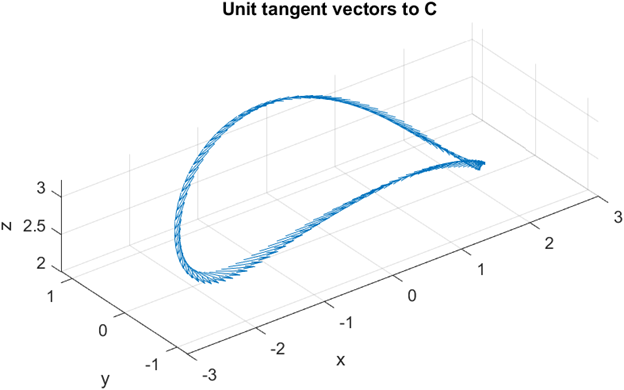
\includegraphics[width=12cm]{graphics/3c.png}
  \caption{Unit tangent vectors to $C$}
\end{figure}

\vspace*{1cm}

Code explanation:
\begin{itemize}
    \item \texttt{\color{mygreen}l = sqrt(x.$\caret$2 + y.$\caret$2 + z.$\caret$2)} - calculates the length of the unit tangent vector at each point on the curve.
    \item \texttt{\color{mygreen}m = -2*sin(t)./l} - calculates the x-component of the unit tangent vector at each point on the curve.
    \item \texttt{\color{mygreen}n = (2/sqrt(3).*cos(t))./l} - calculates the y-component of the unit tangent vector at each point on the curve.
    \item \texttt{\color{mygreen}p = (8.*cos(t).*sin(t))./sqrt(3.*(8.*sin(t).$\caret$2 + 15))./l} - calculates the z-component of the unit tangent vector at each point on the curve.
    \item \texttt{\color{mygreen}quiver3(x\_t, y\_t, z\_t, m, n, p)} - plots the unit tangent vector at each point on the curve as an arrow.
  \end{itemize}
  %\texttt{\color{mygreen}}

\clearpage

\section*{Conclusion}
In conclusion, this assignment has allowed us to delve deeper into the concepts of Calculus 2, including integration techniques. Through three exercises and 
MATLAB problems, we have gained a better understanding of how to apply these concepts in real-world scenarios, and have strengthened our mathematical skills in the process.

In particular, we have learned how to evaluate differnt type of integrals using various methods. We have also studied maximum and mininum values of multivariable functions. Finally, we have investigated various applications of integrals which are arc length, Lagrange Multiplier method, ...

Overall, this assignment has been challenging but rewarding, and has provided us with valuable insights into the power and versatility of Calculus 2. We look forward to continuing our study of this fascinating subject, and applying our newfound knowledge to solve even more complex problems in the future.

% References
\bibliographystyle{plain}
\bibliography{refs/books.bib}
\nocite{*}

\end{document}